% 文档编码: utf-8 
% 创建日期: 2022-02-21 14:46
% 联系作者:  fengzhenhua@outlook.com
% Copyright © 冯振华 .
%
\documentclass[a4paper,fontset = windows]{ctexbook} %Linux 下请自己安装windows,Adobe,found 等相关字体
\usepackage[user=teacher]{cexam}
\usepackage{xeCJKfntef}
\usepackage{xcolor}
\usepackage[margin=2cm]{geometry}
\usepackage{tikz}
\usetikzlibrary{patterns}
\usepackage{float}
\usepackage{amsfonts}
\usepackage{amssymb}
\usepackage{mathtools}
\usepackage{amsthm}
\usepackage{amsmath}
\usepackage{multicol}
\usepackage{graphicx}
%\usepackage{mathpazo}
\usepackage[
  pdfborder=0 0 0,
  bookmarksnumbered=true
]{hyperref}
%\usepackage[user=teacher]{cexam}                   %此宏包为冯振华原创宏包,需要联系作者添加使用
%\usepackage[fontwarning=off]{ctrlwarning}          %此宏包为冯振华原创宏包,用来控制警告信息
%\usepackage{doc}
\usepackage{draftwatermark}
\SetWatermarkText{冯振华}
%\includeonly{                                     %如果使用多个源文档,请取消此注释
%  ,
%}
\begin{document}
\title{\Huge 三维设计(\LaTeX{}版)}
\author{冯振华}
\date{2022年02月21}

\maketitle

%\tableofcontents

\chapter{机械运动}

\section{质点、参考系和坐标系}

\subsubsection{质点}

\begin{jisuan}
   1.下列物体能够看做质点的是
   \qitem 体积很小的原子核
   \qitem 绕太阳公转的地球
   \qitem 用 GPS 确定在大海中位置的航空母舰
   \qitem 正在表演娱乐节目的海狮
   \qitem 研究直升机上正在转动的螺旋桨
   \qitem 研究上坡时有无翻倒可能的三轮车
   \qitem 研究落地时正面朝上还是朝下的硬币
   \qitem 计算北京到上海的火车通过某一路标的时间
\end{jisuan}

\subsubsection{参考系}

\begin{xuanze}
   2.飞机着地后还要在跑道上滑行一段距离,机舱内的乘客透过窗户看到树木向后运动,乘客选择的参考系是
   \choice[A]停在机场的飞机
   \choice[B]候机大楼
   \choice[C]乘客乘坐的飞机
   \choice[D]飞机跑道

   3.第二届青年夏季奥运会于 2014 年 8 月 16 日在南京开幕。观察
   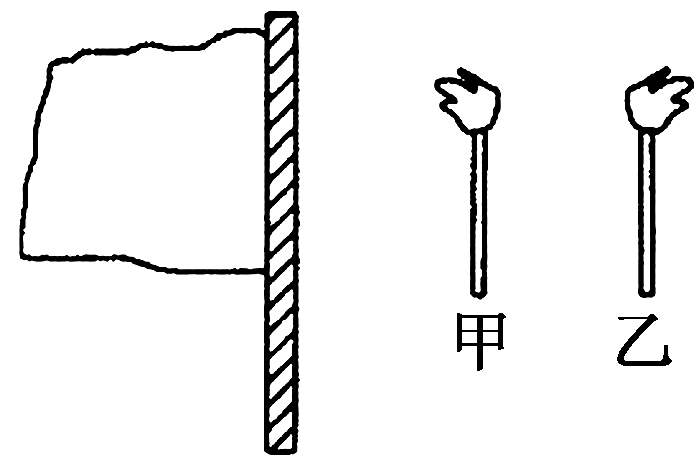
\includegraphics{../picture/1-1/001.png}
   中的旗帜和甲、乙两火炬手所传递的圣火火焰。关于甲、乙两火炬手相对于静止旗杆的运动情况,下列说法中正确的是(旗杆和甲、乙两火炬手在同一地区)
   \choice[A]甲、乙两火炬手一定向左运动
   \choice[B]甲、乙两火炬手一定向右运动
   \choice[C]甲火炬手可能运动,乙火炬手向右运动
   \choice[D]甲火炬手可能静止,乙火炬手向左运动
\end{xuanze}

\subsubsection{位移和路程}

\begin{xuanze}
   4.关于位移和路程,下列说法正确的是()
   \choice[A]在某一段时间内物体运动的位移为零,则该物体一定是静止的
   \choice[B]在某一段时间内物体运动的路程为零,则该物体一定是静止的
   \choice[C]在直线运动中,物体的位移大小一定等于其路程
   \choice[D]在曲线运动中,物体的位移大小可能等于路程

   5.(多选)在机器人大赛中,某机器人在平面内由点(0,0)出发,沿直线运动到点(3,1),然后又由点(3,1)沿直线运动到点(1,4),然后又由点(1,4)沿直线运动到点(5,5),最后又由点(5,5)沿直线运动到点(2,2),平面坐标系横、纵坐标轴的单位长度为 1 m。整个过程中机器人所用时间是 $2\sqrt{2}s$, 则
   \choice[A]机器人的运动轨迹是一条直线
   \choice[B]机器人不会两次通过同一点
   \choice[C]整个过程中机器人的位移大小为 $2\sqrt{2} m$
   \choice[D]整个过程中机器人的位移与由点(5,5)运动到点(2,2)的位移方向相反

\end{xuanze}

\subsubsection{平均速度和瞬时速度}

\begin{xuanze}
   6.如
   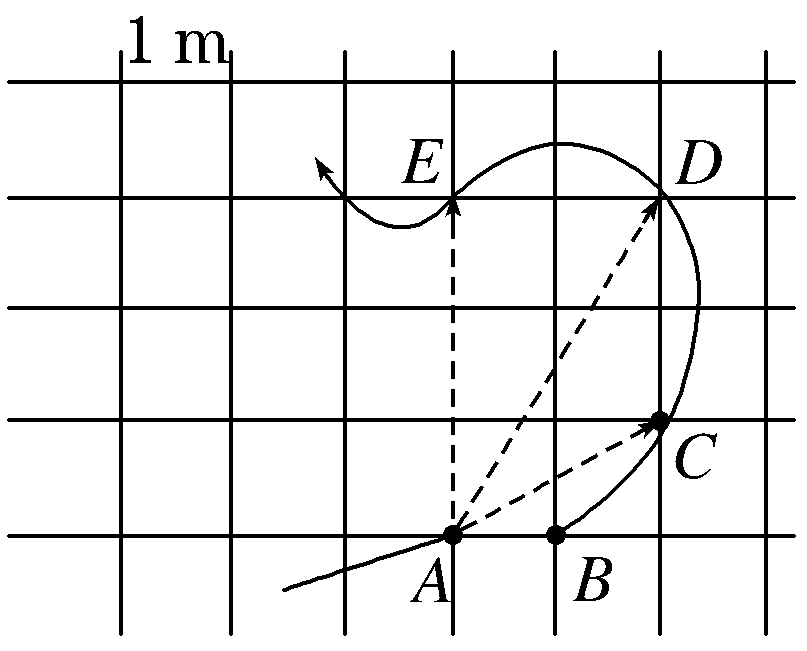
\includegraphics{../picture/1-1/002.png}
   所示,物体沿曲线轨迹的箭头方向运动,AB、ABC、ABCD、ABCDE 四段曲线轨迹运动所用的时间分别是:1 s、2 s、3 s、4 s。下列说法不正确的是
   \choice[A]物体在 AB 段的平均速度为 $1 m/s$
   \choice[B]物体在 ABC 段的平均速度为$ \tfrac{\sqrt{5}}{2} m/s$
   \choice[C]AB 段的平均速度比 ABC 段的平均速度更能反映物体处于 A 点时的瞬时速度
   \choice[D]物体在 B 点的速度等于 AC 段的平均速度

   7.一质点沿直线 Ox 方向做变速运动,它离开 O 点的距离 x 随时间 t 变化的关系为 $x=(5+2t^3)m$,它的速度随时间 t 变化的关系为 $v=6t^2m/s$,该质点在 $t=0$ 到 $t=2 s$ 间的平均速度和 $t=2 s$ 到 $t=3 s$ 间的平均速度的大小分别为
   \choice[A] $12 m/s$\quad $39 m/s$
   \choice[B] $8 m/s$\quad $38 m/s$
   \choice[C] $12 m/s$\quad  $19.5 m/s$
   \choice[D] $8 m/s$\quad $13 m/s$

\end{xuanze}

\begin{jisuan}
   8.为了测定气垫导轨上滑块的加速度,滑块上安装了宽度为 3.0 cm 的遮光板,如
   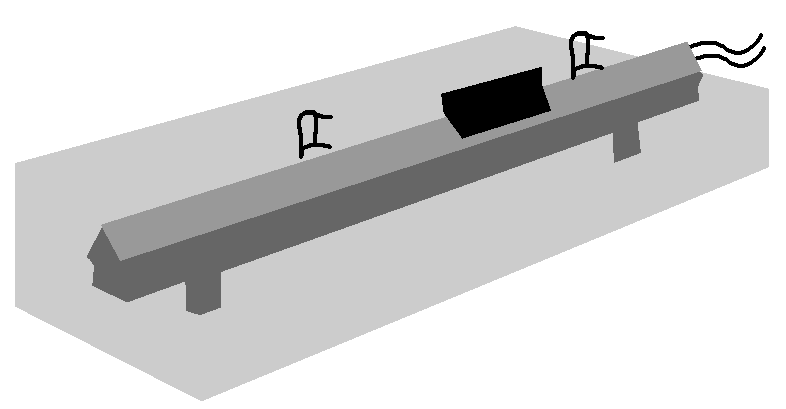
\includegraphics{../picture/1-1/003.png}
所示,滑块在牵引力作用下先后匀加速通过两个光电门,配套的数字毫秒计记录了遮光板通过第一个光电门的时间为$\Delta t_1=0.30 s$,通过第二个光电门的时间为 $\Delta t_2=0.10 s$,遮光板从开始遮住第一个光电门到开始遮住第二个光电门的时间为 $\Delta t=3.0 s$。试估算:
\qitem 滑块的加速度多大(保留两位有效数字)?
\qitem 两个光电门之间的距离是多少?

\end{jisuan}

\subsubsection{速度和加速度}
\begin{xuanze}
   9.下面关于加速度的描述中正确的有
\choice[A]加速度描述了物体速度变化的多少
\choice[B]加速度在数值上等于单位时间里速度的变化量
\choice[C]当加速度与位移方向相反时,物体做减速运动
\choice[D]当加速度与速度方向相同且又减小时,物体做减速运动

10.关于速度、速度的变化和加速度的关系,下列说法中正确的是
\choice[A]速度变化的方向为正,加速度的方向为负
\choice[B]物体加速度增大,速度一定越来越大
\choice[C]速度越来越大,加速度一定越来越大
\choice[D]加速度可能既不与速度同向,也不与速度反向

11.一个质点做速度方向不变的直线运动,加速度的方向始终与速度方向相同,但加速度大小逐渐减小直至为零,在此过程中
\choice[A]速度逐渐减小,当加速度减小到零时,速度达到最小值
\choice[B]速度逐渐增大,当加速度减小到零时,速度达到最大值
\choice[C]位移逐渐增大,当加速度减小到零时,位移将不再增大
\choice[D]位移逐渐减小,当加速度减小到零时,位移达到最小值

12.关于重力加速度,下列说法正确的是
\choice[A]在比萨斜塔上同时由静止释放一大一小两个金属球,两球同时着地,说明两球运动
\choice[B] 速度相同,这个加速度就是当地的重力加速度
\choice[C]地球上各处的重力加速度 g 的值都相同
\choice[D]济南的重力加速度为 $9.8 m/s^2$,说明在济南做下落运动的物体,每经过 $1 s$ 速度增加$9.8 m/s$ 哈尔滨和广州的重力加速度都竖直向下,两者的方向相同

\end{xuanze}


\end{document}
